%%%%%%%%%%%%%%%%%%%%%%%%%%%%%%%%%%%%%%%%%
% Journal Article
% LaTeX Template
% Version 1.3 (9/9/13)
%
% This template has been downloaded from:
% http://www.LaTeXTemplates.com
%
% Original author:
% Frits Wenneker (http://www.howtotex.com)
%
% License:
% CC BY-NC-SA 3.0 (http://creativecommons.org/licenses/by-nc-sa/3.0/)
%
%%%%%%%%%%%%%%%%%%%%%%%%%%%%%%%%%%%%%%%%%

%----------------------------------------------------------------------------------------
%	PACKAGES AND OTHER DOCUMENT CONFIGURATIONS
%----------------------------------------------------------------------------------------

\documentclass[twoside]{article}

\usepackage{lipsum} % Package to generate dummy text throughout this template

\usepackage[sc]{mathpazo} % Use the Palatino font
\usepackage{amsmath}
\usepackage[T1]{fontenc} % Use 8-bit encoding that has 256 glyphs
\linespread{1.05} % Line spacing - Palatino needs more space between lines
\usepackage{microtype} % Slightly tweak font spacing for aesthetics

\usepackage[hmarginratio=1:1,top=32mm,columnsep=20pt]{geometry} % Document margins
\usepackage{multicol} % Used for the two-column layout of the document
\usepackage[hang, small,labelfont=bf,up,textfont=it,up]{caption} % Custom captions under/above floats in tables or figures
\usepackage{booktabs} % Horizontal rules in tables
\usepackage{float} % Required for tables and figures in the multi-column environment - they need to be placed in specific locations with the [H] (e.g. \begin{table}[H])
\usepackage{hyperref} % For hyperlinks in the PDF

\usepackage{lettrine} % The lettrine is the first enlarged letter at the beginning of the text
\usepackage{paralist} % Used for the compactitem environment which makes bullet points with less space between them

\usepackage{abstract} % Allows abstract customization
\renewcommand{\abstractnamefont}{\normalfont\bfseries} % Set the "Abstract" text to bold
\renewcommand{\abstracttextfont}{\normalfont\small\itshape} % Set the abstract itself to small italic text

\usepackage{float}% Places a thin box around figures
\floatstyle{boxed} 
\restylefloat{figure}
\usepackage{graphicx}


\usepackage{titlesec} % Allows customization of titles
\renewcommand\thesection{\Roman{section}} % Roman numerals for the sections
\renewcommand\thesubsection{\Roman{subsection}} % Roman numerals for subsections
\titleformat{\section}[block]{\large\scshape\centering}{\thesection.}{1em}{} % Change the look of the section titles
\titleformat{\subsection}[block]{\large}{\thesubsection.}{1em}{} % Change the look of the section titles

\usepackage{fancyhdr} % Headers and footers
\pagestyle{fancy} % All pages have headers and footers
\fancyhead{} % Blank out the default header
\fancyfoot{} % Blank out the default footer
\fancyhead[C]{Heavy Photon Search Collaboration Note \#XXX} % Custom header text
\fancyfoot[RO,LE]{\thepage} % Custom footer text

\newcommand{\gev}{GeV~}
\newcommand{\mev}{MeV~}

\newcommand{\gevcc}{GeV/c$^2$}
\newcommand{\mevcc}{MeV/c$^2$}
\newcommand{\ap}{A^\prime}
\newcommand{\pos}{e^+}
\newcommand{\ele}{e^-}
\newcommand{\trifull}{\ele~W\to\ele\ele\pos~W}
\newcommand{\apfull}{\ele~W\to\ele\ap(\to\ele\pos)~W}
\newcommand{\epem}{\pos\ele}




%----------------------------------------------------------------------------------------
%	TITLE SECTION
%----------------------------------------------------------------------------------------

\title{\vspace{-15mm}\fontsize{24pt}{10pt}\selectfont\textbf{Trident Cross-section Measurement for the 2015 Engineering Run @ 1.05 GeV}} % Article title
\author{
\large
\textsc{Matt Graham} % Your name
\normalsize SLAC\\ % Your institution
\normalsize \href{mailto:mgraham@slac.stanford.edu}{mgraham@slac.stanford.edu} % Your email address
\vspace{0mm}
}
\date{\today}

%----------------------------------------------------------------------------------------

\begin{document}


\maketitle % Insert title

\thispagestyle{fancy} % All pages have headers and footers

%----------------------------------------------------------------------------------------
%	ABSTRACT
%----------------------------------------------------------------------------------------

\begin{abstract}
We describe the reconstruction, selection, and cross-section determination of $\trifull$, i.e. "tridents".  This analysis reconstructs $\ele\pos$ pairs from data taken during the 1.05 \gev running in spring 2015.  We compare the measured cross-sections and kinematic distributions between data and MC. 
\noindent % \lipsum[1] % Dummy abstract text
\end{abstract}

%----------------------------------------------------------------------------------------
%	ARTICLE CONTENTS
%----------------------------------------------------------------------------------------

%\begin{multicols}{2} % Two-column layout throughout the main article text

\section{Introduction}

At the amplitude level, there are two diagrams (at the lowest order) which contribute to "trident" (i.e. 3-prong) final states when scattering an electron beam off a nuclear target:  Bethe-Heitler (BH) and radiative diagrams\ref{fig:feynman}.  Both of these amplitudes (and their interference) contribute to the background in the dark photon ($\ap$) search.  

The BH background has a huge amplitude but very different kinematics than the $\ap$ reaction and can be significantly, but not completely, suppressed by making appropriate phase space cuts.

The radiative reaction, however, has identical kinematics to the $\ap$ reaction 
$\apfull$ and the rate of $\ap$ production is related to the radiative production via: 
\begin{equation}
\sigma(\ap)=X \sigma(rad).
\end{equation}
Verifying the radiative cross-section that is observed by HPS is an important confirmation that the experiment is working as designed and is also a key input to setting mass-coupling limits for $\ap$ detection.  

This note describes the reconstruction, selection, and methods used to extract the trident cross-section as well as a number of cross-checks performed.  

%\begin{figure}[tbh]
%  \centering
%      \includegraphics[width=0.5\textwidth]{feynman-diags.pdf}
%  \caption{Straight line fit to the leading edge of the RF signal.}
%  \label{fig:feynman}
%\end{figure}	



%\lettrine[nindent=0em,lines=3]{T}  
%------------------------------------------------

\section{Datasets}

Below we summarize the datasets used in this study.  


\begin{itemize}
\item Data
\begin{itemize}
\item reconstruction pass-2.1, DST v0.8.1 unblind sample
\end{itemize}
\item Monte Carlo:  using HPS-EngineeringRun2015-v3 with pass-2 reconstruction
\begin{itemize}
\item pure samples
\begin{itemize}
\item \textbf{Full amplitude tridents}:  MadGraph generation includes BH+radiative interference.  Generator-level cuts:  blahblah; 
\item \textbf{Radiative tridents}:  MadGraph generation.  Generator-level cuts:  blahblah;
\item \textbf{Bethe-Heitler tridents}:  MadGraph generation.  Generator-level cuts:  blahblah;
\end{itemize}
\end{itemize}
\end{itemize}

Summarize some stuff about the MC generations, readout and recon. 

\begin{table}[htdp]
\caption{default}
\begin{center}
\begin{tabular}{c|c|c|c}
\hline
Sample    			&Generated       & Number     & Pair1\\
				& Cross-Section& Generated & Acceptance\\
\hline
Full Tridents		&  1.76mb		 &  16560k      & 0.126  \\
Radiative Tridents 	&  	0.12mb	 &  3000k	      &  0.129 \\
BH Tridents		&  8.28mb		&  5000k***	& 0.022\\
\hline
Full w/pileup		&   1.76mb	& 87.7k		& 0.141\\
\hline
\end{tabular}
\end{center}
\label{tab:mc}
\end{table}%

%\begin{figure}[H]
%  \centering
%      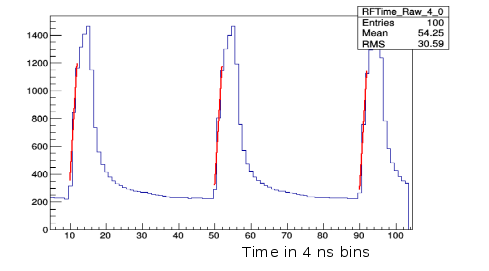
\includegraphics[width=0.5\textwidth]{rfFitting.png}
%  \caption{Straight line fit to the leading edge of the RF signal.}
%  \label{rfsignal}
%\end{figure}	

%\begin{figure}[H]
%  \centering
%      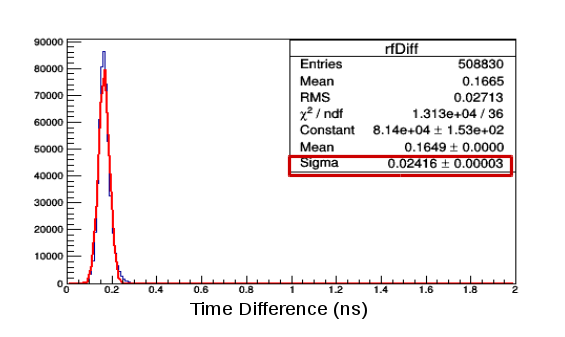
\includegraphics[width=0.5\textwidth]{rfRes.png}
%  \caption{Time difference between the RF signal in the two different FADC channels.}
%  \label{rfresolution}
%\end{figure}

%------------------------------------------------

\section{Reconstruction}

The data and MC both use the pass-2 reconstruction (release???)  but with the correction (bug) that was effecting the momenta and invariant mass of fitted $\epem$ pairs.  We will update this to an official pass as soon as it is available.  The reconstruction chain is described briefly below. 

The tracking reconstruction follows this chain: 
\begin{itemize}
\item for each strip hit recorded, the six ADC samples from the APV25 chip are fit to extract the time and amplitude
\item on each sensor, neighboring strip hits are clustered together, defining a strip cluster
\item hits on stereo pair sensors are combined to make a hit in 3D space
\item a seed of a track is created by fitting a helix to hits in 3 layers iterating, over all hits in those layers
\item hits in subsequent layers are added to the seed and either added to the track or rejected depending on goodness of fit and whether it pulls the track too far from the beamspot at the target
\item multiple combinations of seeding layers are used to ensure good efficiency
\end{itemize}
The tracking efficiency has been shown to be $>95\%$ (I hope!), using a combination of Moller events and full-energy electrons \cite{effNote}. More detail on the tracking reconstruction can be found in Reference \cite{trackingNote}.

Similar for ECal recon and SVT-ecal matching.   




\section{Event Selection \& Efficiency}

At this stage of analysis, we've chose to keep cuts simple and fairly loose.  Below, we list the criteria used for selecting trident candidates: 
\begin{itemize}
\item pass the  pairs-1 trigger; the fraction of events passing this trigger is listed in Table \ref{tab:mc}. 
\item N($\pos$)=1
\item  0<N($\ele$)<5
\item the event must have at least 1 $\epem$ pair (a "V0") satisfying the following cuts:
\begin{itemize}
\item unconstrained vertex fit $\chi^2<10$
\item unconstrained fitted Z-momentum: $0.6<p_z<1.3~\gev$
\item unconstrained fitted vertex position:  $|V_x|<2~mm$; $|V_y|<2~mm$; $|V_z|<25~mm$
\item $50<p<900~\mev$ for both tracks
\item $p(\pos)\times p(\ele)<0$ (top-bottom pairs)
\end{itemize}
\item the number of V0 candidates cuts = 1
\end{itemize}

Nice table with cut-by-cut efficiency for different samples. 



\section{Cross-Section Calculation}

\subsection{Integrated Luminosity \& Live Time}

Discussion on how lumi and livetime  is calculated...

\subsection{Cross-Section Results}

Discussion on how XS is calculated...

Nice table of results comparing MC and data 

Run-by-run XS plot

\section{Kinematic Distribution Comparisons}

Some plot and discussion of plots


\begin{figure}[htbp]
  \centering
      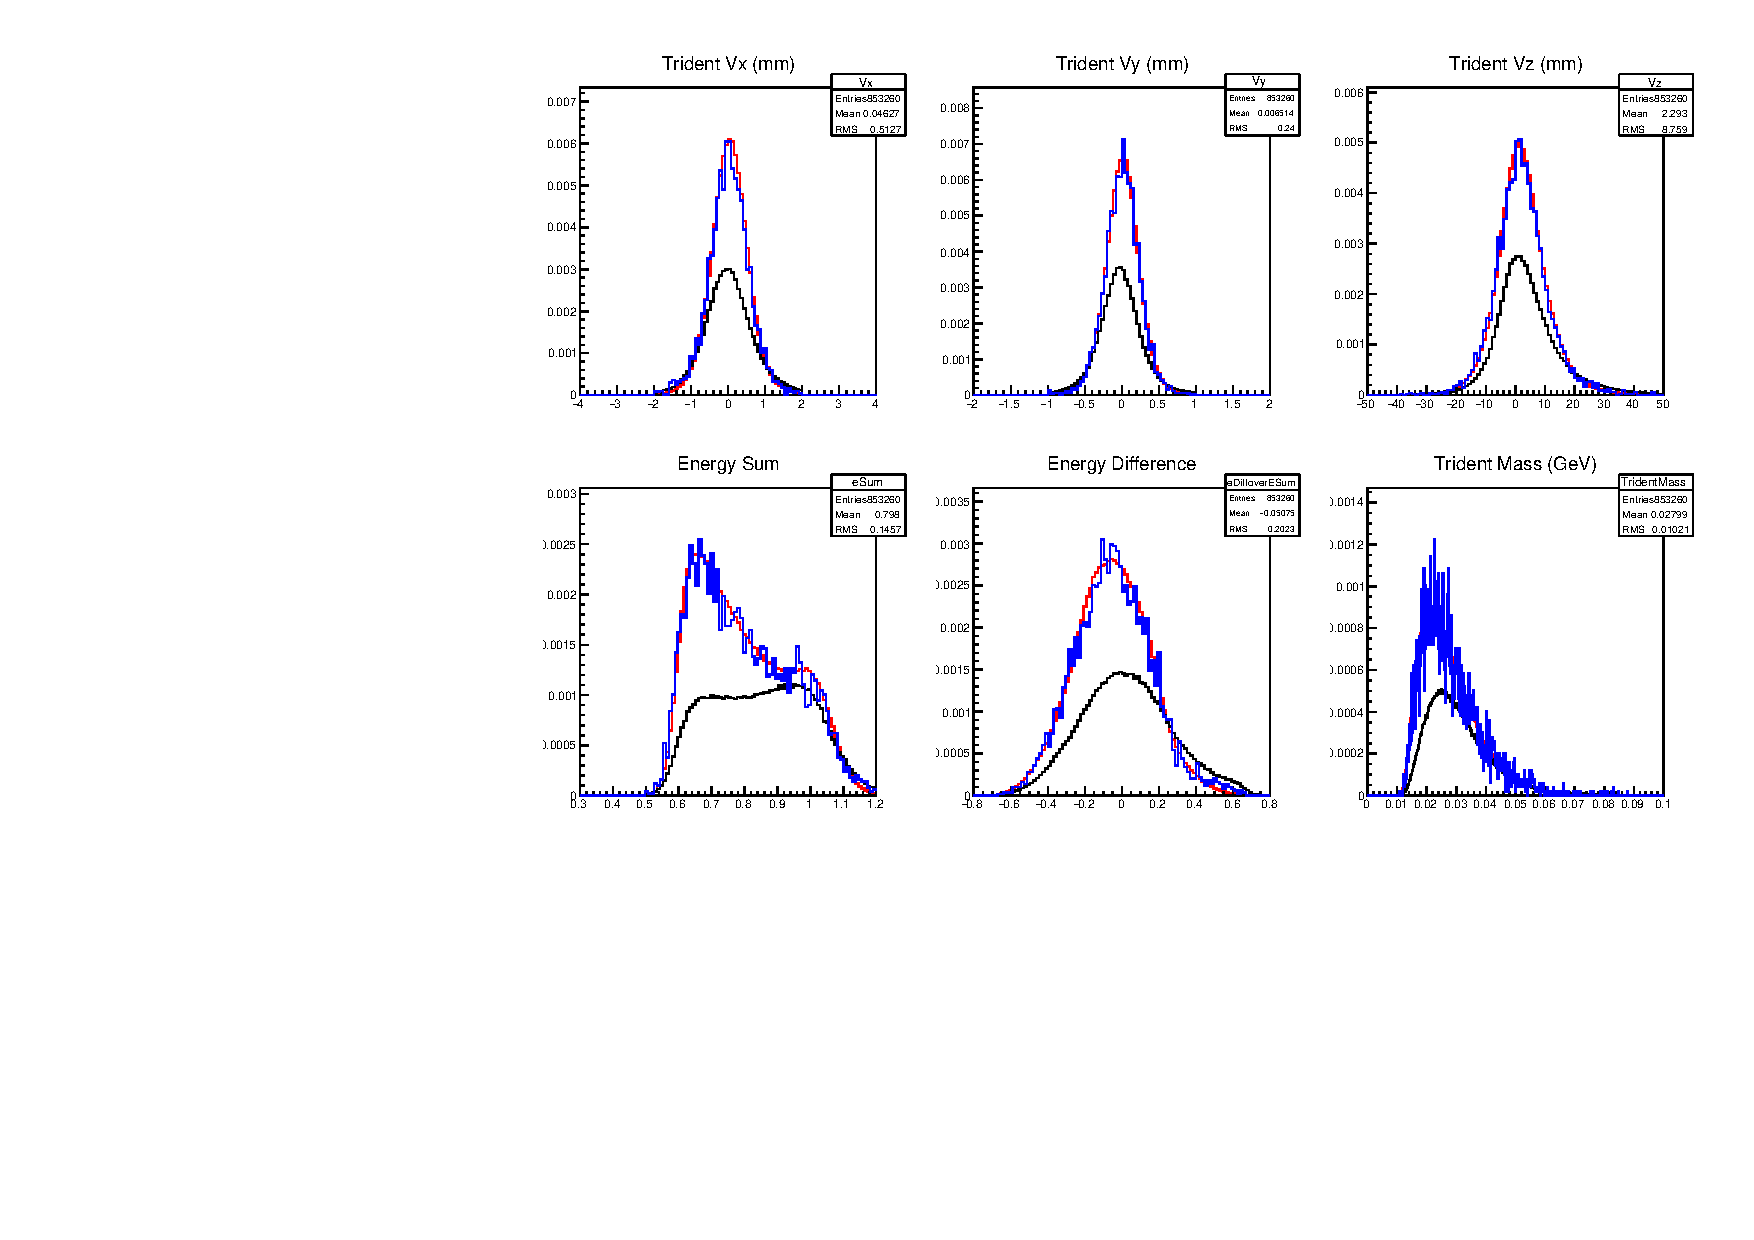
\includegraphics[width=0.9\textwidth]{v0summary-norm-to-XS.pdf}
  \caption{Make nicer plots!!!}
  \label{rfsignal}
\end{figure}	



\section{Conclusion}

Wrap it up

%----------------------------------------------------------------------------------------
%	REFERENCE LIST
%----------------------------------------------------------------------------------------

\begin{thebibliography}{99} % Bibliography - this is intentionally simple in this template
\end{thebibliography}

%----------------------------------------------------------------------------------------

%\end{multicols}

\end{document}
